\documentclass[12pt] {article}
\usepackage{times}
\usepackage[margin=1in,bottom=1in,top=0.6in]{geometry}

\usepackage{hhline}
\usepackage{subfig}
\usepackage{amsmath}
\usepackage{amsfonts}
\usepackage[inline,shortlabels]{enumitem}%enumerate with letters
\usepackage{mathrsfs} 
\usepackage[square,numbers]{natbib}
\usepackage{graphicx}
\bibliographystyle{unsrtnat}
\usepackage{float}
\usepackage[dvipsnames]{xcolor}
\usepackage{tikz}
\usepackage{amsfonts,amsmath, color, fullpage, graphicx, mathtools, empheq, amsthm, amssymb}
\usepackage{wasysym}
\usepackage{thmtools}
\usepackage{listings}
\usepackage[ruled,vlined, linesnumbered]{algorithm2e}
\usepackage{flexisym}
\usepackage{breqn}
\setenumerate[0]{label=(\alph*)}

\usepackage[framed,numbered,autolinebreaks,useliterate]{../../mcode}

%To write numbers in scientific notation nicely
%use as \expnumber{2.000000000000000}{+00} to write 2.000000000000000e+00
\newcommand{\expnumber}[2]{{#1}\mathrm{e}{#2}}



\begin{document}

\title{MAT 226B – Large Scale Matrix Computation \\ Final Project}
\author{Ahmed Mahmoud}
\date{March, 22nd 2020} 

\maketitle




%============Table========
%\begin{figure}[tbh]
% \centering    
%\begin{tabular}{ |p{4cm}|| p{2cm}|p{2cm}|p{2cm}|p{2cm}|}
% \hline
% & Processor 1 &  Processor 2  & Processor 3 & Processor 4\\ \hhline{|=|=|=|=|=|}
% \hline
% Performance          &$1.08$        &$1.425$       &\textbf{1.52}  &   \\
% \hline
%\end{tabular} 
%\caption{Metric table for the four processors}
%   \label{tab:metric}
%\end{figure} 
%============Figure========
%\begin{figure}[!tbh]
%\centering        
%   \subfloat {\includegraphics[width=0.65\textwidth]{fig2_4.png}}
%   \caption{ }
%   \label{fig:fig}
%\end{figure}
%============Code========
%\begin{lstlisting}
%function [f,g] = linear_regression(theta, X,y)
%end
%\end{lstlisting}


\newpage
\section*{Problem 1:}

\section*{Problem 2:}
Here we are required to find an efficient way to compute $q = Mv$ and $q = M^{T}v$ for $v \in \mathbb{C}^{n}$ where $M = (A - s_{0}E)^{-1}E$. We can compute the matrix-vector multiplication efficiently using LU factorization. We first can write the multiplication as

\begin{align*}
& q = (A-s_{0}E)^{-1}Ev = (\underbrace{A-s_{0}E}_{W})^{-1}\underbrace{Ev}_{f} \\
& q = W^{-1} f \quad \Rightarrow \quad Wq = f \quad \Rightarrow \quad \underbrace{PD^{-1}WQ}_{LU}\underbrace{Q^{T}q}_{d} = PD^{-1}f \\
\end{align*}
Thus, we can fist solve $Lc = PD^{-1}f$ for $c \in \mathbb{C}^{n}$ via forward substitution, then solve $Ud = c$ for $d \in \mathbb{C}^{n}$ via backward substitution, and finally set $q = Qd$. 

We can use the same LU factorization to compute $q = M^{T}v$ efficiently. We first not that transposing the LU factorization for a given matrix $W$ is $U^{T}L^{T} = Q^{T}W^{T}D^{-T}P^{T}$
 We can write this multiplication as 

\begin{align*}
& q = ((A-s_{0}E)^{-1}E)^{T}v = E^{T}\underbrace{(A-s_{0}E)^{-T}v}_{g}\\
& g = W^{-T} v \quad \Rightarrow \quad W^{T}g = v \quad \Rightarrow \quad \underbrace{Q^{T}W^{T}D^{-T}P^{T}}_{U^{T}L^{T}}\underbrace{(D^{-T}P^{T})^{-1}g}_{d}=Q^{T}v\\
\end{align*}

Thus, we can first solve $U^{T}c = Q^{T}v$ for $c$ via forward substitution, then solve $L^{T}d = c$ for $d$ via backward substitution, and then set $g = D^{-T}P^{T}d$. Finally, we multiply $g$ from the left by $E^{T}$ to get $q$. The functions \texttt{Mv} and \texttt{transposeMv} implements these operations as discussed. 


\newpage
\section*{Problem 3:}
\begin{enumerate}
\item Function \texttt{hermitian\_lanczos} implements the Hermitian Lanczos process where it takes the matrix $A$, vector $r$, and \texttt{KMAX} parameter and output $T_{k}$ tridiagonal matrix in sparse format. We used this function to approximate eigenvalues of $A$ from \texttt{make\_3d\_laplacian} function using $k=7$. Table~\ref{tab:app_eig_7} shows the results where the first two columns show the exact eigenvalues of $A$ (computed from the provided function) along its multiplicity and last column shows the approximate eigenvalues. We can see that the approximate solution is able to capture all the eigenvalues with very high accuracy.

\begin{figure}[tbh]
 \centering    
\begin{tabular}{ |p{5cm}| p{2cm}|| p{5cm}|}
\hline
 Exact Eigenvalues  & Multiplicity & Approximate Eigenvalues \\ \hhline{|=|=|=|}   
$\expnumber{1.757359312880715}{+00}$ & 1& $\expnumber{1.757359312880715}{+00}$ \\
$\expnumber{3.171572875253810}{+00}$ &3 & $\expnumber{3.171572875253810}{+00}$ \\
$\expnumber{4.585786437626905}{+00}$ &6 & $\expnumber{4.585786437626905}{+00}$ \\
$\expnumber{6.000000000000000}{+00}$ & 7& $\expnumber{6.000000000000002}{+00}$ \\
$\expnumber{7.414213562373095}{+00}$&6 & $\expnumber{7.414213562373095}{+00}$ \\
$\expnumber{8.828427124746190}{+00}$ &3 & $\expnumber{8.828427124746192}{+00}$ \\
$\expnumber{1.024264068711928}{+01}$ &1 & $\expnumber{1.024264068711929}{+01}$ \\
\hline
\end{tabular} 
\caption{Exact and approximate eigenvalues using Hermitian Lanczos process}
   \label{tab:app_eig_7}
\end{figure}

\item We used \texttt{hermitian\_lanczos} to compute the approximate eigenvalues for the 262144 \times 262144 matrix from \texttt{make\_3d\_laplacian(64)}. Tables~\ref{tab:app_eig_100,tab:app_eig_200,tab:app_eig_400,tab:app_eig_800,tab:app_eig_1200, tab:app_eig_1600,tab:app_eig_2000} show the 10 smallest and 10 largest approximated eigenvalues. Table~\ref{tab:exact_64} shows the 10 smallest and 10 largest exact eigenvalues. 

\begin{figure}[tbh]
 \centering    
\begin{tabular}{ ||p{6cm}||p{6cm}|}
\hline
 Smallest Eigenvalues & Largest Eigenvalues \\ \hhline{|=|=|}   
\hline
$\expnumber{1.422787575075167}{-02}$ & $\expnumber{1.170222368514153}{+01}$ \\  
$\expnumber{2.522292134967839}{-02}$ & $\expnumber{1.175506886438500}{+01}$ \\  
$\expnumber{3.720946521956244}{-02}$ & $\expnumber{1.180683457939747}{+01}$ \\  
$\expnumber{6.015341020592301}{-02}$ & $\expnumber{1.184896392339356}{+01}$ \\  
$\expnumber{8.407846117839080}{-02}$ & $\expnumber{1.188540931980204}{+01}$ \\  
$\expnumber{1.168498457907536}{-01}$ & $\expnumber{1.191749739736500}{+01}$ \\  
$\expnumber{1.581734700307590}{-01}$ & $\expnumber{1.194638621492721}{+01}$ \\  
$\expnumber{1.995732825474702}{-01}$ & $\expnumber{1.196512279467138}{+01}$ \\  
$\expnumber{2.466691832816189}{-01}$ & $\expnumber{1.198055273500129}{+01}$ \\  
$\expnumber{3.011244810109077}{-01}$ & $\expnumber{1.199293004521624}{+01}$ \\  
\hline  
\end{tabular} 
\caption{Approximate Eigenvalues using $K = 100$}
   \label{tab:app_eig_100}
\end{figure} 


\begin{figure}[tbh]
 \centering    
\begin{tabular}{ ||p{6cm}||p{6cm}|}
\hline
 Smallest Eigenvalues & Largest Eigenvalues \\ \hhline{|=|=|}   
\hline
$\expnumber{7.006926067695284}{-03}$ & $\expnumber{1.191194541966088}{+01}$ \\  
$\expnumber{1.400816296330363}{-02}$ & $\expnumber{1.192367820060319}{+01}$ \\  
$\expnumber{2.104749654401042}{-02}$ & $\expnumber{1.193815033138952}{+01}$ \\  
$\expnumber{2.644416419643677}{-02}$ & $\expnumber{1.194943725586547}{+01}$ \\  
$\expnumber{3.252921177956383}{-02}$ & $\expnumber{1.195823115974695}{+01}$ \\  
$\expnumber{4.248144987518579}{-02}$ & $\expnumber{1.196722905407029}{+01}$ \\  
$\expnumber{5.158180541911261}{-02}$ & $\expnumber{1.197279443138257}{+01}$ \\  
$\expnumber{6.175958581860198}{-02}$ & $\expnumber{1.197897280487774}{+01}$ \\  
$\expnumber{7.373377938324976}{-02}$ & $\expnumber{1.198599186623671}{+01}$ \\  
$\expnumber{8.527634111033579}{-02}$ & $\expnumber{1.199299336087879}{+01}$ \\  
\hline  
\end{tabular} 
\caption{Approximate Eigenvalues using $K = 200$}
   \label{tab:app_eig_200}
\end{figure} 

\begin{figure}[tbh]
 \centering    
\begin{tabular}{ ||p{6cm}||p{6cm}|}
\hline
 Smallest Eigenvalues & Largest Eigenvalues \\ \hhline{|=|=|}    
\hline
$\expnumber{7.006639006043782}{-03}$ & $\expnumber{1.195105825040107}{+01}$ \\  
$\expnumber{1.400782323540659}{-02}$ & $\expnumber{1.195568924396476}{+01}$ \\  
$\expnumber{2.100900746475762}{-02}$ & $\expnumber{1.195806895929420}{+01}$ \\  
$\expnumber{2.565829376859278}{-02}$ & $\expnumber{1.196033932970904}{+01}$ \\  
$\expnumber{2.801019169415529}{-02}$ & $\expnumber{1.196734052200119}{+01}$ \\  
$\expnumber{3.265947799840193}{-02}$ & $\expnumber{1.197198980830585}{+01}$ \\  
$\expnumber{3.966069944862968}{-02}$ & $\expnumber{1.197434170623140}{+01}$ \\  
$\expnumber{4.193108831261764}{-02}$ & $\expnumber{1.197899099253526}{+01}$ \\  
$\expnumber{4.431079048315387}{-02}$ & $\expnumber{1.198599217676459}{+01}$ \\  
$\expnumber{4.897191625334762}{-02}$ & $\expnumber{1.199299336099394}{+01}$ \\  
\hline  
\end{tabular} 
\caption{Approximate Eigenvalues using $K = 400$}
   \label{tab:app_eig_400}
\end{figure} 

\begin{figure}[tbh]
 \centering    
\begin{tabular}{ ||p{6cm}||p{6cm}|}
\hline
 Smallest Eigenvalues & Largest Eigenvalues \\ \hhline{|=|=|}    
\hline
$\expnumber{7.006639006040011}{-03}$ & $\expnumber{1.197198980830589}{+01}$ \\  
$\expnumber{7.006639006045063}{-03}$ & $\expnumber{1.197434170555307}{+01}$ \\  
$\expnumber{1.400782323539451}{-02}$ & $\expnumber{1.197434170623140}{+01}$ \\  
$\expnumber{1.400782323540438}{-02}$ & $\expnumber{1.197899099253525}{+01}$ \\  
$\expnumber{2.100900746475027}{-02}$ & $\expnumber{1.197899099253527}{+01}$ \\  
$\expnumber{2.100900746475296}{-02}$ & $\expnumber{1.198599217676461}{+01}$ \\  
$\expnumber{2.565829371816093}{-02}$ & $\expnumber{1.198599217676461}{+01}$ \\  
$\expnumber{2.565829376859185}{-02}$ & $\expnumber{1.199293916949044}{+01}$ \\  
$\expnumber{2.801018851772900}{-02}$ & $\expnumber{1.199299336099396}{+01}$ \\  
$\expnumber{2.801019169410766}{-02}$ & $\expnumber{1.199299336099397}{+01}$ \\  
\hline  
\end{tabular} 
\caption{Approximate Eigenvalues using $K = 800$}
   \label{tab:app_eig_800}
\end{figure} 

\begin{figure}[tbh]
 \centering    
\begin{tabular}{ ||p{6cm}||p{6cm}|}
\hline
 Smallest Eigenvalues & Largest Eigenvalues \\ \hhline{|=|=|}   
\hline
$\expnumber{7.006639006034983}{-03}$ & $\expnumber{1.197899099253524}{+01}$ \\  
$\expnumber{7.006639006042774}{-03}$ & $\expnumber{1.197899099253525}{+01}$ \\  
$\expnumber{7.006639006050910}{-03}$ & $\expnumber{1.197899099253525}{+01}$ \\  
$\expnumber{7.006642433917978}{-03}$ & $\expnumber{1.198599217676460}{+01}$ \\  
$\expnumber{1.400782323538701}{-02}$ & $\expnumber{1.198599217676461}{+01}$ \\  
$\expnumber{1.400782323539747}{-02}$ & $\expnumber{1.198599217676462}{+01}$ \\  
$\expnumber{1.400782323539999}{-02}$ & $\expnumber{1.199299336099394}{+01}$ \\  
$\expnumber{2.100900746475157}{-02}$ & $\expnumber{1.199299336099396}{+01}$ \\  
$\expnumber{2.100900746475692}{-02}$ & $\expnumber{1.199299336099397}{+01}$ \\  
$\expnumber{2.100900746476310}{-02}$ & $\expnumber{1.199299336099399}{+01}$ \\  
\hline  
\end{tabular} 
\caption{Approximate Eigenvalues using $K = 1200$}
   \label{tab:app_eig_1200}
\end{figure} 

\begin{figure}[tbh]
 \centering    
\begin{tabular}{ ||p{6cm}||p{6cm}|}
\hline
 Smallest Eigenvalues & Largest Eigenvalues \\ \hhline{|=|=|}     
\hline
$\expnumber{7.006639006034724}{-03}$ & $\expnumber{1.197899099253525}{+01}$ \\  
$\expnumber{7.006639006037083}{-03}$ & $\expnumber{1.198599217676456}{+01}$ \\  
$\expnumber{7.006639006037985}{-03}$ & $\expnumber{1.198599217676460}{+01}$ \\  
$\expnumber{7.006639006044512}{-03}$ & $\expnumber{1.198599217676460}{+01}$ \\  
$\expnumber{7.006639006047808}{-03}$ & $\expnumber{1.198599217676461}{+01}$ \\  
$\expnumber{1.400782323539137}{-02}$ & $\expnumber{1.199299336099392}{+01}$ \\  
$\expnumber{1.400782323539370}{-02}$ & $\expnumber{1.199299336099395}{+01}$ \\  
$\expnumber{1.400782323539474}{-02}$ & $\expnumber{1.199299336099396}{+01}$ \\  
$\expnumber{1.400782323540451}{-02}$ & $\expnumber{1.199299336099397}{+01}$ \\  
$\expnumber{1.412781215190661}{-02}$ & $\expnumber{1.199299336099398}{+01}$ \\  
\hline  
\end{tabular} 
\caption{Approximate Eigenvalues using $K = 1600$}
   \label{tab:app_eig_1600}
\end{figure} 

\begin{figure}[tbh]
 \centering    
\begin{tabular}{ ||p{6cm}||p{6cm}|}
\hline
 Smallest Eigenvalues & Largest Eigenvalues \\ \hhline{|=|=|}    
\hline
$\expnumber{7.006639006032009}{-03}$ & $\expnumber{1.198599217676460}{+01}$ \\  
$\expnumber{7.006639006034958}{-03}$ & $\expnumber{1.198599217676460}{+01}$ \\  
$\expnumber{7.006639006035550}{-03}$ & $\expnumber{1.198599217676461}{+01}$ \\  
$\expnumber{7.006639006037528}{-03}$ & $\expnumber{1.198599260901220}{+01}$ \\  
$\expnumber{7.006639006037725}{-03}$ & $\expnumber{1.199299336099394}{+01}$ \\  
$\expnumber{7.006639006042897}{-03}$ & $\expnumber{1.199299336099395}{+01}$ \\  
$\expnumber{1.400782323536894}{-02}$ & $\expnumber{1.199299336099396}{+01}$ \\  
$\expnumber{1.400782323539092}{-02}$ & $\expnumber{1.199299336099396}{+01}$ \\  
$\expnumber{1.400782323539872}{-02}$ & $\expnumber{1.199299336099396}{+01}$ \\  
$\expnumber{1.400782323540259}{-02}$ & $\expnumber{1.199299336099397}{+01}$ \\  
\hline  
\end{tabular} 
\caption{Approximate Eigenvalues using $K = 2000$}
   \label{tab:app_eig_2000}
\end{figure} 


\begin{figure}[tbh]
 \centering    
\begin{tabular}{ ||p{6cm}||p{6cm}|}
\hline
 Smallest Eigenvalues & Largest Eigenvalues \\ \hhline{|=|=|}    
\hline
$\expnumber{7.006639006040594}{-03}$ & $\expnumber{1.197434170623141}{+01}$ \\  
$\expnumber{1.400782323539662}{-02}$ & $\expnumber{1.197434170623141}{+01}$ \\  
$\expnumber{1.400782323539662}{-02}$ & $\expnumber{1.197434170623141}{+01}$ \\  
$\expnumber{1.400782323539662}{-02}$ & $\expnumber{1.197899099253525}{+01}$ \\  
$\expnumber{2.100900746475265}{-02}$ & $\expnumber{1.197899099253525}{+01}$ \\  
$\expnumber{2.100900746475265}{-02}$ & $\expnumber{1.197899099253525}{+01}$ \\  
$\expnumber{2.100900746475265}{-02}$ & $\expnumber{1.198599217676460}{+01}$ \\  
$\expnumber{2.565829376859075}{-02}$ & $\expnumber{1.198599217676460}{+01}$ \\  
$\expnumber{2.565829376859163}{-02}$ & $\expnumber{1.198599217676460}{+01}$ \\  
$\expnumber{2.565829376859163}{-02}$ & $\expnumber{1.199299336099396}{+01}$ \\  
\hline  
\end{tabular} 
\caption{Exact Eigenvalues}
   \label{tab:exact_64}
\end{figure} 

\end{enumerate}
\newpage
\section*{Problem 4:}

\noindent
Figure \ref{fig:problem_4} shows the associated graph $G(A)$ of matrix $A$ along with the steps of the minimum degree algorithm. From these steps, the reordering of the nodes will be $2, 4, 5, 3, 6, 7, 1, 8, 9$



\begin{figure}[!tbh]
\centering        
   \subfloat{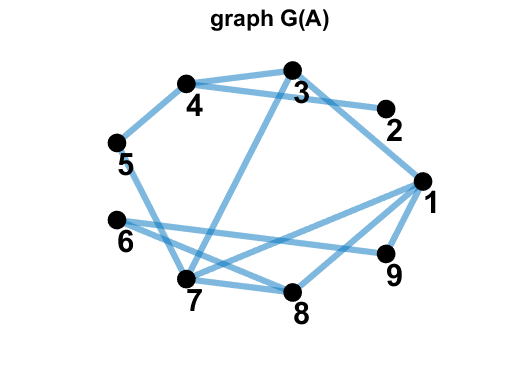
\includegraphics[width=0.33\textwidth]{../code/0.png}}
   \subfloat{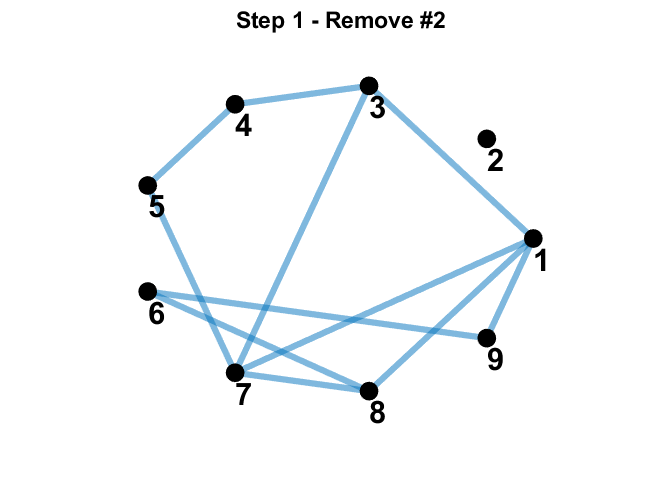
\includegraphics[width=0.33\textwidth]{../code/1.png}}   
   \subfloat{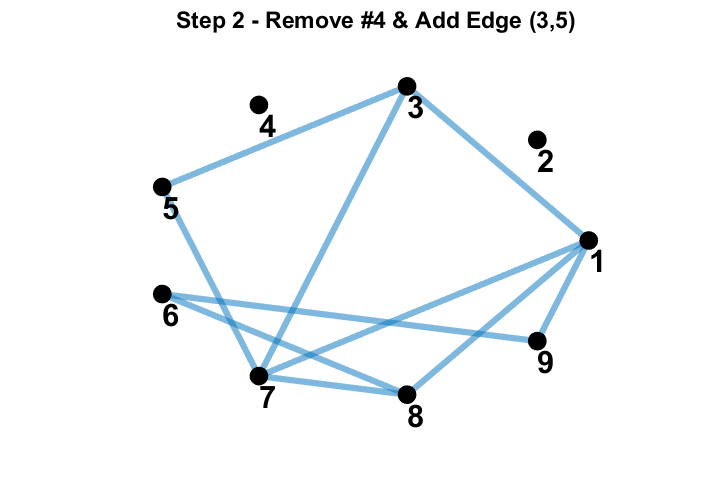
\includegraphics[width=0.33\textwidth]{../code/2.png}}
    
   \subfloat{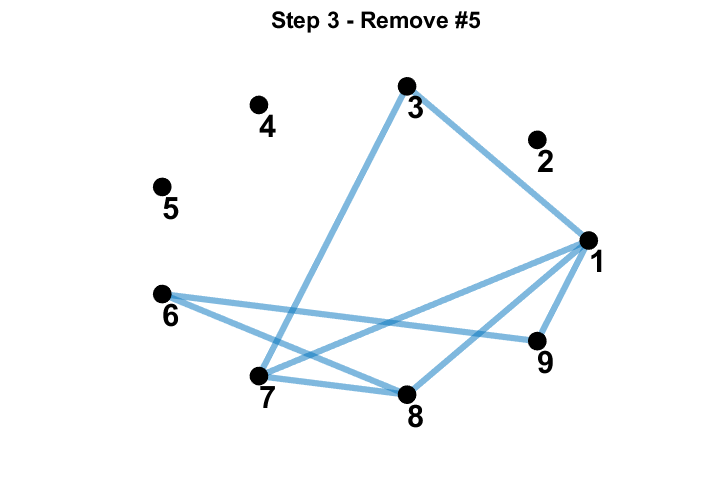
\includegraphics[width=0.33\textwidth]{../code/3.png}}
   \subfloat{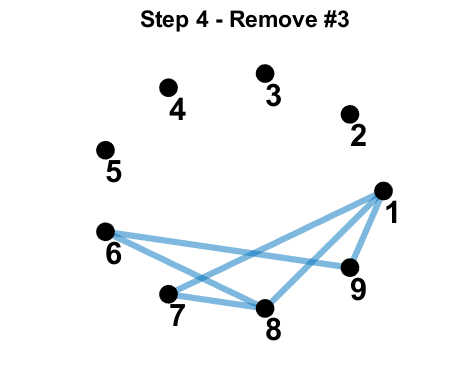
\includegraphics[width=0.33\textwidth]{../code/4.png}}
   \subfloat{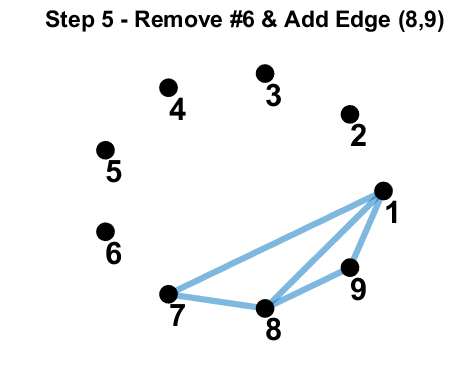
\includegraphics[width=0.33\textwidth]{../code/5.png}}
   
   \subfloat{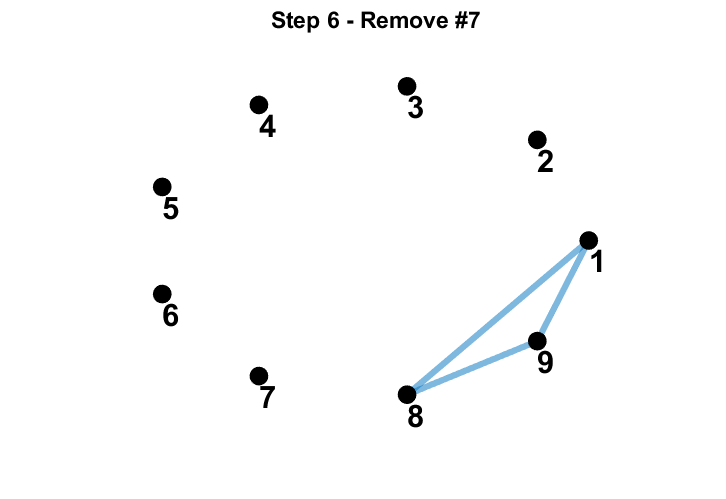
\includegraphics[width=0.33\textwidth]{../code/6.png}}
   \subfloat{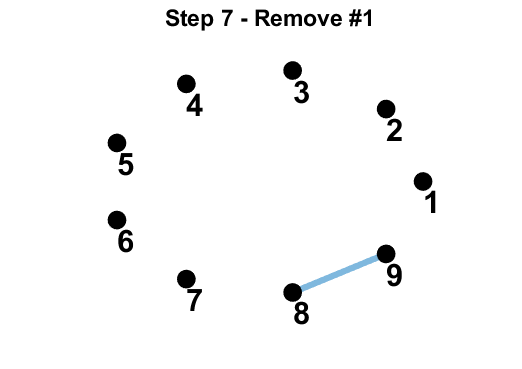
\includegraphics[width=0.33\textwidth]{../code/7.png}}
   \subfloat{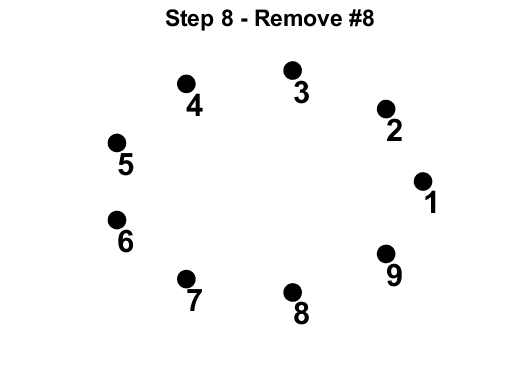
\includegraphics[width=0.33\textwidth]{../code/8.png}}
   \caption{Graph $G(A)$ along with the 8 steps of the minimum degree algorithm applied on it. }
   \label{fig:problem_4}
\end{figure}

\noindent
From the reordering above, the permutation matrix can be constructed such that 

$$
P = 
\begin{bmatrix}
0 & 0 & 0 & 0 & 0 & 0 & 1 & 0 & 0\\
1 & 0 & 0 & 0 & 0 & 0 & 0 & 0 & 0\\
0 & 0 & 0 & 1 & 0 & 0 & 0 & 0 & 0\\
0 & 1 & 0 & 0 & 0 & 0 & 0 & 0 & 0\\
0 & 0 & 1 & 0 & 0 & 0 & 0 & 0 & 0\\
0 & 0 & 0 & 0 & 1 & 0 & 0 & 0 & 0\\
0 & 0 & 0 & 0 & 0 & 1 & 0 & 0 & 0\\
0 & 0 & 0 & 0 & 0 & 0 & 0 & 1 & 0\\
0 & 0 & 0 & 0 & 0 & 0 & 0 & 0 & 1\\
\end{bmatrix}
$$

\noindent
From which, we can compute $P^{T}AP$ to be

$$
P^{T}AP = 
\begin{bmatrix}
* & * & 0 & 0 & 0 & 0 & 0 & 0 & 0 \\
* & * & * & * & 0 & 0 & 0 & 0 & 0 \\
0 & * & * & 0 & 0 & * & 0 & 0 & 0 \\
0 & * & 0 & * & 0 & * & * & 0 & 0 \\
0 & 0 & 0 & 0 & * & 0 & 0 & * & * \\
0 & 0 & * & * & 0 & * & * & * & 0 \\
0 & 0 & 0 & * & 0 & * & * & * & * \\
0 & 0 & 0 & 0 & * & * & * & * & 0 \\
0 & 0 & 0 & 0 & * & 0 & * & 0 & * \\
\end{bmatrix}
$$

\noindent
Applying Cholesky factorization to $P^{T}AP$ we get the following lower triangular matrix where the fill-in elements are shown with $\color{red}{+}$

$$
L = 
\begin{bmatrix}
* & 0 & 0 & 0 & 0 & 0 & 0 & 0 & 0 \\
* & * & 0 & 0 & 0 & 0 & 0 & 0 & 0 \\
0 & * & * & 0 & 0 & 0 & 0 & 0 & 0 \\
0 & * & \color{red}{+} & * & 0 & 0 & 0 & 0 & 0 \\
0 & 0 & 0 & 0 & * & 0 & 0 & 0 & 0 \\
0 & 0 & * & * & 0 & * & 0 & 0 & 0 \\
0 & 0 & 0 & * & 0 & * & * & 0 & 0 \\
0 & 0 & 0 & 0 & * & * & * & * & 0 \\
0 & 0 & 0 & 0 & * & 0 & * & \color{red}{+} & * \\
\end{bmatrix}
$$

\section*{Problem 5:}
\paragraph{System Specs:} All our experiments run on Intel(R) Xeon(R) CPU E3-1280 v5 with 3.70 GHz and 32 GB of RAM on 64-bit operating system running Windows 7. 

\paragraph{Plots:} Figure~\ref{fig:all} shows the results of the three algorithms plotted on top of each others. It shows that Lanczos-based algorithm is able to capture $Z(s)$ almost exactly using $k=100$. For such value of $k$, the textbook algorithm will return NaN everywhere. Thus, we used $k=10$ in the plot. Function \texttt{Figure\_1()} in \texttt{driver.m} file generates this plot. 

\begin{figure}[!tbh]
\centering        
   \subfloat {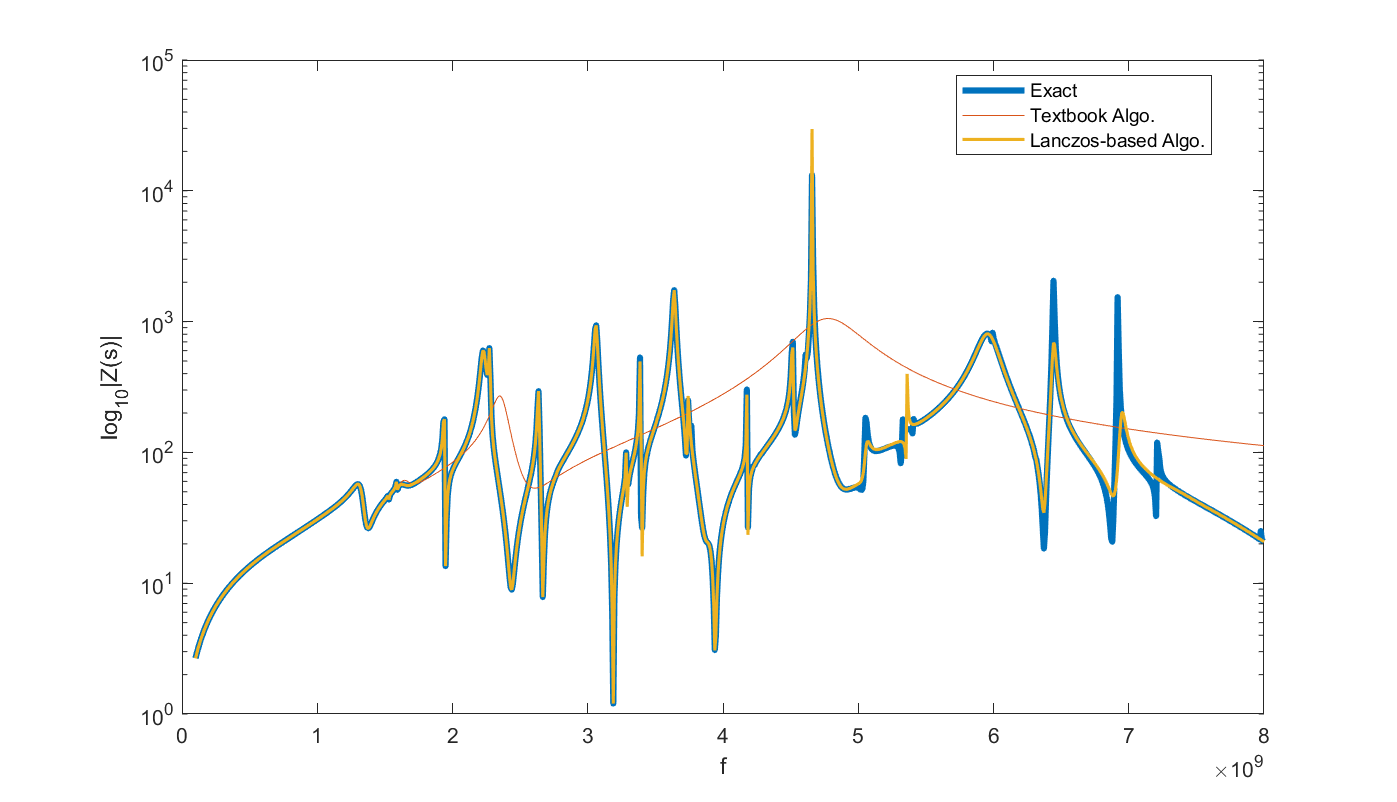
\includegraphics[width=0.85\textwidth]{../code/figure1.png}}
   \caption{The results of the three algorithms; exact algorithm, textbook algorithm with $k=10$, and Lanczos-based algorithm with $k=100$. We used expansion point $s_{0} = \expnumber{1}{5} + 2\pi i \expnumber{5.5}{8}$ for both algorithms.   }
   \label{fig:all}
\end{figure}

\paragraph{$s_0$ with fast convergence:} We test our implementation of the textbook and Lanczos-based algorithm for different values of $s_{0}$ and found that it runs fairly fast for the small input given in \texttt{FP\_Ex1.mat}; it takes less than a second even for large i.e., $k < 100$. 

We followed the recommendation given in the lectures for how to pick $s_{0}$. We choose $s_{0} = \expnumber{1}{5} + 2\pi i \expnumber{5.5}{8} $. 

\paragraph{Comparison:} We run both our implementation for different values of $k$ and the above $s_{0}$ and compared between both. Table~\ref{tab:comp} shows the average different ($\parallel \cdot \parallel^{2}$) and the maximum (absolute) different between the two vectors containing the output of both algorithms for different values of $s$. Function \texttt{Table\_1()} in \texttt{driver.m} file generates these data. We can see that when $k>13$, the two algorithms will give difference numerical results. 

\begin{table}[!tbh]
 \centering    
\begin{tabular}{ |p{1.5cm}| p{4cm}|| p{4cm}|}
\hline
 $k$  & Average Difference & Maximum Difference \\ \hhline{|=|=|=|}   
    2   & $\expnumber{2.082747}{-28}$   & $\expnumber{2.109424}{-15}$   \\
	3   & $\expnumber{7.919421}{-27}$   & $\expnumber{6.439294}{-15}$   \\
	4   & $\expnumber{5.026520}{-25}$   & $\expnumber{4.618528}{-14}$   \\
	5   & $\expnumber{8.547583}{-26}$   & $\expnumber{2.664535}{-14}$   \\
	6   & $\expnumber{3.052289}{-23}$   & $\expnumber{4.112266}{-13}$   \\
	7   & $\expnumber{1.148403}{-19}$   & $\expnumber{4.235057}{-11}$   \\
	8   & $\expnumber{2.656897}{-17}$   & $\expnumber{3.190033}{-09}$   \\
	9   & $\expnumber{6.690131}{-15}$   & $\expnumber{1.812676}{-08}$   \\
	10  & $\expnumber{6.292776}{-12}$   & $\expnumber{3.008865}{-07}$   \\
	11  & $\expnumber{7.619719}{-11}$   & $\expnumber{6.315981}{-06}$   \\
	12  & $\expnumber{4.360106}{-04}$   & $\expnumber{1.650155}{-02}$   \\
	13  & $\expnumber{9.107709}{-04}$   & $\expnumber{1.494378}{-02}$   \\
	14  & $\expnumber{7.052574}{+00}$   & $\expnumber{3.945073}{-01}$   \\
	15  & $\expnumber{5.904627}{+01}$   & $\expnumber{1.279984}{+00}$   \\
	16  & $\expnumber{1.779754}{+02}$   & $\expnumber{1.488481}{+00}$   \\
	17  & $\expnumber{1.105689}{+02}$   & $\expnumber{1.625567}{+00}$   \\
	18  & $\expnumber{1.100795}{+02}$   & $\expnumber{1.632208}{+00}$   \\
	19  & $\expnumber{1.219843}{+02}$   & $\expnumber{1.688382}{+00}$   \\
	20  & $\expnumber{1.075413}{+02}$   & $\expnumber{9.725151}{-01}$   \\
	21  & $\expnumber{1.108709}{+02}$   & $\expnumber{1.217680}{+00}$   \\
	22  & $\expnumber{4.712087}{+02}$   & $\expnumber{1.762950}{+00}$   \\
	23  & $\expnumber{1.160591}{+03}$   & $\expnumber{2.593543}{+00}$   \\
	24  & $\expnumber{3.507356}{+03}$   & $\expnumber{4.102138}{+00}$   \\
	25  & $\expnumber{7.329648}{+03}$   & $\expnumber{5.568756}{+00}$   \\
	26  & $\expnumber{2.245490}{+04}$   & $\expnumber{8.889336}{+00}$   \\
	27  & $\expnumber{2.633420}{+04}$   & $\expnumber{9.681861}{+00}$   \\
	28  & $\expnumber{4.881768}{+04}$   & $\expnumber{1.252447}{+01}$   \\
	29  & $\expnumber{7.066637}{+04}$   & $\expnumber{1.471937}{+01}$   \\
	30  & $\expnumber{1.151561}{+05}$   & $\expnumber{1.801101}{+01}$   \\
\hline
\end{tabular} 
\caption{Average and maximum (absolute) difference between the results of the textbook algorithm and Lanczos approach for different $k$ values.}
   \label{tab:comp}
\end{table}

\paragraph{Explanation:} We believe the reason why the textbook algorithm does not perform well is because it depends on computing $M^{j}r$ (to compute the moments) for increasing values of $j$ which convergences quickly to the the eigenvector of $M$ with largest eigenvalue. Thus, the information it contains comes from a single eigenvector where the information should comes from all eigenvectors of $M$. In contrast, Lanczos's $T_{k}$ represents oblique projection of $M$ onto the $K_{k}(M,r)$ Krylov subspace which contains information about $k$ eigenvectors. 

\paragraph{Lanczos approach with difference $s_{0}$:} For this experiment, we defined the ``good approximation'' such that the average difference between the Lanczos-based algorithm and the exact algorithm is less than  $10^{-5}$. We tested using different $s_{0}$ and for each value we run the algorithm in a loop for $200\leq k \leq 1000$ and stop when the results meet the good-approximation criterion we set thus obtaining the minimum $k$ value that results into the best approximation given $s_{0}$. Table~\ref{tab:s0} show the results for different $s_{0}$. Function \texttt{Table\_2()} in \texttt{driver.m} file generates these data.

We notice that complex $s_{0}$ take more time for the same $k$ value (first and last row in Table~\ref{tab:s0}. Expansion point with complex part equal to the maximum or minimum frequency take double the time it takes for $s_{0}$ suggested in the lecture notes. Getting closer y-axis can results in higher $k$ values and thus slower convergence. 


\begin{table}[!tbh]
 \centering    
\begin{tabular}{ |p{3.0cm}|p{1.5cm}| p{4cm}|| p{4cm}|}
\hline
 $s_{0}$  & $k$ & Time & Average Difference \\ \hhline{|=|=|=|=|}   
 $10^{5} + 2 \pi i f_{avg}$  & 212 & 3.416422 & $\expnumber{7.9513}{-6}$\\
 $10^{5} + 2 \pi i f_{min}$ & 278 & 7.300847 & $\expnumber{6.419988}{-6}$\\
 $10^{5} + 2 \pi i f_{max}$ & 262 & 6.130839 & $\expnumber{8.102979}{-7}$ \\
 $10^{9} $                  & 290 & 6.739243 & $\expnumber{8.396701}{-6}$ \\
 $10^{10}$                  & 212 & 2.901619 & $\expnumber{4.187281}{-6}$  \\  
\hline
\end{tabular} 
\caption{Lanczos approach using different $k$ and $s_{0}$ values and comparing it with the exact solution ($f_{avg} = \frac{f_{min}+f_{max}}{2}$) }
   \label{tab:s0}
\end{table}
\section*{Problem 6:}




\end{document}
